\pdfminorversion=4
\documentclass[]{beamer}
\mode<presentation>

% beamer stuff
% Gives us the bottom line with all the goodies
\useoutertheme{infolines}
% Just the theme to use. Should be built into bemaer. Setting the
% height gets rid of a whole lot of whitespace
\usetheme[height=7mm]{Rochester}
\usefonttheme{serif}
% Usually beamer gives you navigation hyperlinks on the bottom
% right. I turned this off. It's annoying.
\setbeamertemplate{navigation symbols}{} 
% Makes my text boxes look pretty
\setbeamertemplate{blocks}[rounded][shadow=true] 
% Makes my bullet points 3d balls
\setbeamertemplate{items}[ball]

% Josh's packages
\usepackage{multimedia}
\usepackage{graphicx}

% Packages for me
\usepackage{amsmath,amssymb,latexsym,amsthm}
\usepackage[mathscr]{eucal}
\usepackage{mathrsfs}
\usepackage{verbatim}
\usepackage{braket}
\usepackage{listings}
\usepackage{xcolor}
% \usepackage[usenames,dvipsnames,svgnames,table]{xcolor}
\usepackage{fancybox}
\usepackage{animate}
% \usepackage{media9}
\usepackage{multicol}
\usepackage{mdframed}
\usepackage{hyperref}
%\usepackage{scalerel}
\usepackage[outline]{contour}
\contourlength{1.2pt}

% Macros

%Blackboard Bold
\newcommand{\R}{\mathbb{R}}
\newcommand{\Z}{\mathbb{Z}}
\newcommand{\N}{\mathbb{N}}
\newcommand{\Q}{\mathbb{Q}}
\newcommand{\A}{\mathbb{A}}
\newcommand{\E}{\mathbb{E}}
% other
\newcommand{\eval}{\biggr\rvert} %evaluated at
\newcommand{\myvec}[1]{\mathbf{#1}} % vectors for me
% total derivatives 
\newcommand{\diff}[2]{\frac{d #1}{d #2}} 
\newcommand{\dd}[1]{\frac{d}{d #1}}
% partial derivatives
\newcommand{\pd}[2]{\frac{\partial #1}{\partial #2}} 
\newcommand{\pdd}[1]{\frac{\partial}{\partial #1}} 
% Order operator
\DeclareRobustCommand{\orderof}{\ensuremath{\mathcal{O}}}

% braces
\newcommand{\paren}[1]{\left( #1 \right)}
\newcommand{\sqrbrace}[1]{\left[ #1 \right]}
\newcommand{\curlybrace}[1]{\left\{ #1 \right\}}
\newcommand{\inner}[1]{\paren{#1}}
\newcommand{\norm}[1]{\left| #1 \right|_2}

% g
\newcommand{\detg}{\sqrt{-g}}

% neutrinos
\newcommand{\eepsilon}{\epsilon} % energy
\newcommand{\fin}{f\in \{\nu_e,\nu_{\bar{e}},\nu_x\}}
\newcommand{\sign}{\text{sign}(f)}
\newcommand{\jnuf}{j_{\eepsilon,f}}
\newcommand{\etanuf}{\eta_{\eepsilon,f}}
\newcommand{\Inuf}{I_{\eepsilon,f}}
\newcommand{\chinuf}{\chi_{\eepsilon,f}}
\newcommand{\sigmanuf}{\sigma_{\eepsilon,f}}
\newcommand{\alphanuf}{\alpha_{\eepsilon,f}}
\newcommand{\numin}{\nu_{\text{min}}}
\newcommand{\numax}{\nu_{\text{max}}}


% tikz
\usepackage{tikz}
\usepackage{pgfplots}
\usetikzlibrary{calc,fadings,decorations.pathreplacing}
\usetikzlibrary{arrows}
\usetikzlibrary{decorations.pathmorphing}
\usetikzlibrary{decorations.markings}
\usetikzlibrary{arrows.meta,bending}

% Keys to support piece-wise uncovering of elements in TikZ pictures:
% \node[visible on=<2->](foo){Foo}
% \node[visible on=<{2,4}>](bar){Bar}   % put braces around comma expressions
% 
% Internally works by setting opacity=0 when invisible, which has the 
% adavantage (compared to \node<2->(foo){Foo} that the node is always there, hence
% always consumes space plus that coordinate (foo) is always available.
% 
% The actual command that implements the invisibility can be overriden
% by altering the style invisible. For instance \tikzsset{invisible/.style={opacity=0.2}}
% would dim the "invisible" parts. Alternatively, the color might be set to white, if the
% output driver does not support transparencies (e.g., PS) 
% 
\tikzset{
  invisible/.style={opacity=0},
  visible on/.style={alt={#1{}{invisible}}},
  alt/.code args={<#1>#2#3}{%
    \alt<#1>{\pgfkeysalso{#2}}{\pgfkeysalso{#3}} % \pgfkeysalso doesn't change the path
  },
}

% some nice flowchart features
\tikzset{
    mynode/.style={rectangle,rounded corners,draw=black, top color=white, bottom color=yellow!50,very thick, inner sep=1em, minimum size=3em, text centered},
    myimgnode/.style={rectangle,rounded corners,draw=black, top color=white, bottom color=yellow!50,very thick, inner sep=0.25em, minimum size=3em, text centered},
    myarrow/.style={->, >=latex', shorten >=2pt, thick},
    mylabel/.style={text width=8em, text centered} 
}  

% squigly arrow
\tikzset{zigzag it/.style={decorate, decoration=zigzag}}

% Color morphing arrow
\tikzset{colormorph/.style n args={3}{
    postaction={
    decorate,
    decoration={
    markings,
    mark=between positions 0 and \pgfdecoratedpathlength step 0.5pt with {
    \pgfmathsetmacro\myval{multiply(
        divide(
        \pgfkeysvalueof{/pgf/decoration/mark info/distance from start}, \pgfdecoratedpathlength
        ),
        100
    )};
    \pgfsetfillcolor{#3!\myval!#2};
    \pgfpathcircle{\pgfpointorigin}{#1};
    \pgfusepath{fill};}
}}}}

% define a really nice visible "purple"
\definecolor{gimppurple}{HTML}{AD26FB}
% a light grey
\definecolor{lightgrey}{HTML}{E0E0E0}
% for highlighting
\definecolor{deepblue}{rgb}{0,0,0.5}
\definecolor{deepred}{rgb}{0.6,0,0}
\definecolor{deepgreen}{rgb}{0,0.5,0}

% fonts
% Default fixed font does not support bold face
\DeclareFixedFont{\ttb}{T1}{txtt}{bx}{n}{12} % for bold
\DeclareFixedFont{\ttm}{T1}{txtt}{m}{n}{12}  % for normal

% Python style for highlighting
\newcommand\pythonstyle{\lstset{
language=Python,
basicstyle=\ttm,
otherkeywords={self},
keywordstyle=\ttb\color{deepblue},
emph={__init__},           
emphstyle=\ttb\color{deepred},
commentstyle=\ttfamily\color{deepred},
stringstyle=\color{deepgreen},
frame=tb,                     
showstringspaces=false        
}}

% Python environment
\lstnewenvironment{python}[1][]
{
\pythonstyle
\lstset{#1}
}
{}

\newcommand{\backupbegin}{
   \newcounter{finalframe}
   \setcounter{finalframe}{\value{framenumber}}
}
\newcommand{\backupend}{
   \setcounter{framenumber}{\value{finalframe}}
}

% Automatically generates section breaker slides
\AtBeginSection[]{
  \begin{frame}[plain]
  \vfill
  \centering
  \begin{beamercolorbox}[sep=8pt,center,shadow=true,rounded=true]{title}
    \usebeamerfont{title}\insertsectionhead\par%
  \end{beamercolorbox}
  \vfill
  \end{frame}
}

\title[NSM$\nu$]{How full neutrino transport impacts heavy element
  formation in the universe and the resulting electromagnetic
  counterpart}
% \subtitle{Models and Implications}
\author[J. Miller]{\textcolor{blue}{Jonah M. Miller}, \color{black}in collaboration with:\\
  \color{red}Brandon Barker, Kelsey Lund,\\ Mariam Gogilashvili\\
\color{black}And Many More...}
\institute[LANL]{Los Alamos National Laboratory}
% \titlegraphic{\vspace{1cm}}
% \titlegraphic{\includegraphics[height=0.25\textheight]{3d_render}}
% \date[9/19/19]{LA Astro Seminar}
\date[ET]{Einstein Toolkit Workshop}

\graphicspath{{figures/}}

\begin{document}

\begin{frame}[plain]
    \tikz [remember picture, overlay] 
    \node at ([xshift=2cm,yshift=-2cm]current page.west)
    {\includegraphics[width=0.25\textwidth,clip,trim={150 0 150 0}]{3d_render}};
    \tikz [remember picture, overlay] 
    \node at ([xshift=-2cm,yshift=-2cm]current page.east)
    {\includegraphics[width=0.25\textwidth,clip,trim={0 0 0 0}]{visit0006-gimp3}};
  \titlepage
\end{frame}

\begin{frame}[plain]
  This should be a conversation! 
  \begin{itemize}
  \item Please feel free to interrupt me and ask questions as I speak.
  \item I plan to leave lots of time for questions.
  \end{itemize}
  The required legalese:
  \begin{itemize}
  \item This Document cleared for unlimited release with
    LA-UR-24-25455
  \item The submitted materials have been authored by an employee or
    employees of Triad National Security, LLC (Triad) under contract
    with the U.S.  Department of Energy/National Nuclear Security
    Administration (DOE/NNSA).  Accordingly, the U.S. Government
    retains an irrevocable, nonexclusive, royalty- free license to
    publish, translate, reproduce, use, or dispose of the published
    form of the work and to authorize others to do the same for
    U.S. Government purposes.”
  \end{itemize}
\end{frame}

\begin{frame}
  \frametitle{Neutron Star Mergers: A 2+ Component Model}
  \begin{columns}
    \begin{column}{6cm}
      \begin{center}
        % \includegraphics[width=0.9\textwidth]{frames/betabin_000}
        \animategraphics[width=0.9\textwidth,every=10,autoplay,loop,controls]
        {5}{frames/betabin_}{000}{374}
      \end{center}
    \end{column}
    \begin{column}{6cm}
      \begin{center}
        \resizebox{\columnwidth}{!}{
          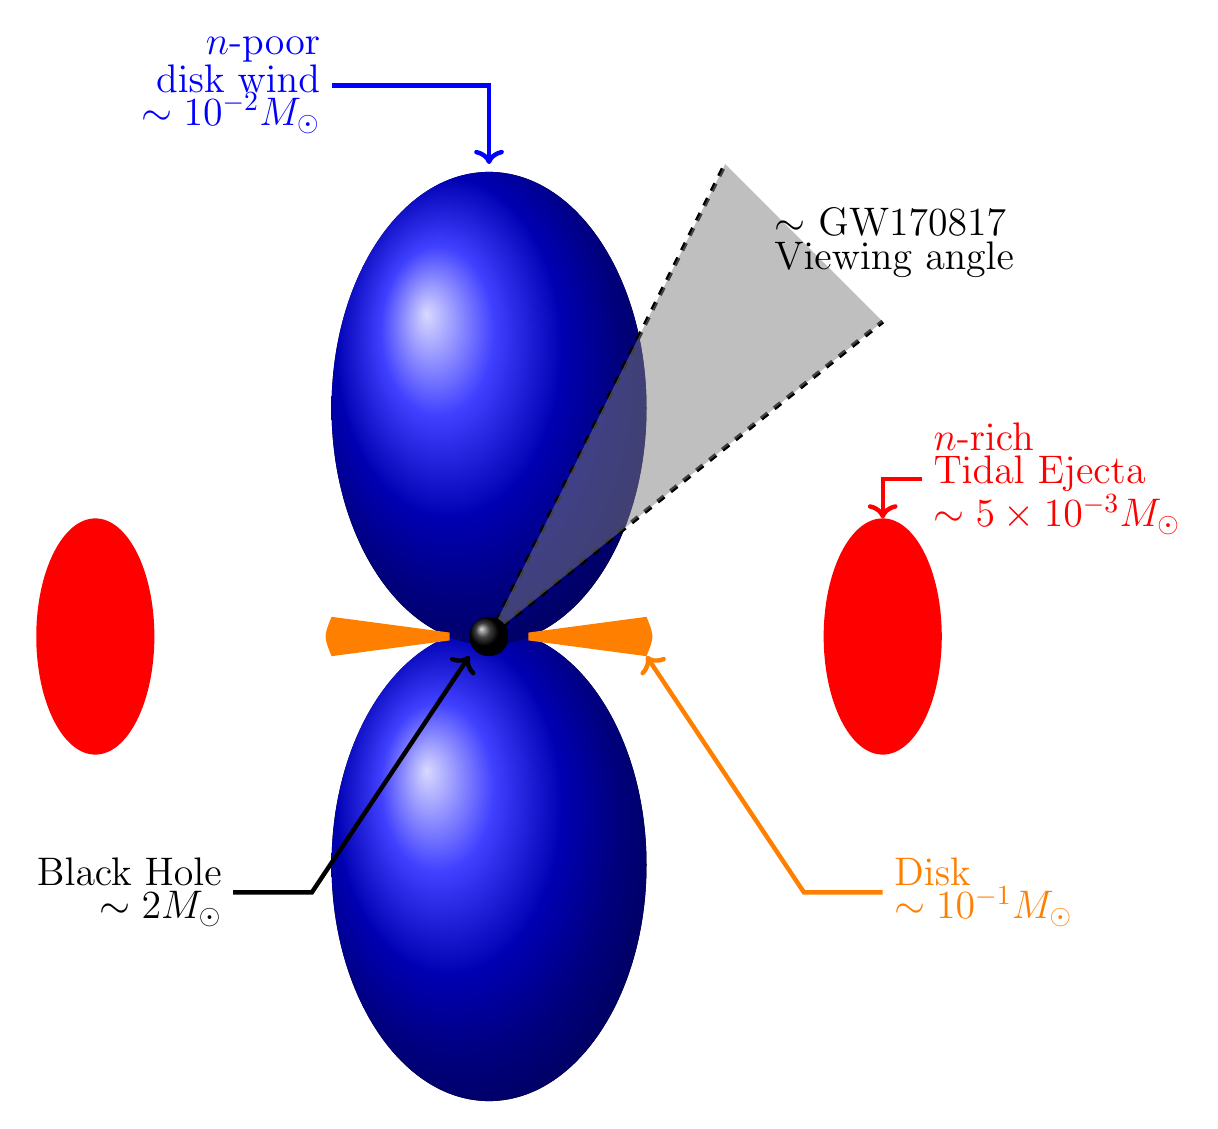
\begin{tikzpicture}
            \coordinate (origin) at (0,0);
            \pgfmathsetmacro{\dbx}{0.5}
            \pgfmathsetmacro{\dby}{0.05}
            \pgfmathsetmacro{\dex}{2.}
            \pgfmathsetmacro{\dey}{0.25}
            \pgfmathsetmacro{\dcc}{2.1}
            \pgfmathsetmacro{\tcx}{5.0}

            \foreach \i in {-1,1}
            {
              \fill[ball color=blue] (0, \i*2.9) ellipse (2 and 3);
            }

            \foreach \i in {-1,1}
            {
              % disk
              \fill[color=orange]
              (\i*\dbx,\dby) -- (\i*\dex,\dey)
              .. controls (\i*\dcc,0) .. (\i*\dex,-\dey)
              -- (\i*\dbx,-\dby) -- cycle;

              % tidal ejecta
              \fill[color=red] (\i*\tcx,0) ellipse (0.75 and 1.5);
            }

            % viewing
            \draw[dashed,ultra thick,black] (origin) -- (5,4);
            \draw[dashed,ultra thick,black] (origin) -- (3,6);
            \fill[color=gray,opacity=0.5] (origin) -- (5,4) -- (3,6) -- cycle;
            \node[right,align=left] at (3.5,5)
            {\Large $\sim$ GW170817\\ \Large Viewing angle};

            % bh
            \shade[ball color=black] (origin) circle (0.25);

            % text
            \draw[<-,red, ultra thick] (\tcx,1.5)
            -- ++(0.,0.5) -- ++(0.5,0)
            node[right,align=left]
            {\Large \color{red}$n$-rich\\\Large Tidal Ejecta\\ \Large $\sim 5\times 10^{-3}M_{\odot}$};

            \draw[<-,blue, ultra thick] (0,6) -- ++(0,1) -- ++(-2,0)
            node[left,align=right]
            {\Large \color{blue}$n$-poor\\\Large disk wind\\\Large $\sim 10^{-2}M_{\odot}$};

            \draw[<-,orange, ultra thick] (\dex,-\dey)
            -- ++(2,-3) -- ++(1,0)
            node[right,align=left]
            {\Large \color{orange}Disk\\\Large $\sim 10^{-1}M_{\odot}$};

            \draw[<-,black, ultra thick] (-0.25,-0.25)
            -- ++(-2,-3) -- ++(-1,0)
            node[left,align=right]
            {\Large \color{black}Black Hole\\ \Large $\sim 2 M_{\odot}$};
          \end{tikzpicture}
        }
      \end{center}
    \end{column}
  \end{columns}
  \begin{tiny}
    Co-design summer school, 2016
  \end{tiny}
\end{frame}

\begin{frame}
  \frametitle{The r-process}
  \begin{center}
   \includegraphics[width=0.9\textwidth]{skynet_ye_0p13/frame_0001}
  \end{center}
  Courtesy of J. Lippuner
\end{frame}

\begin{frame}
  \frametitle{The r-process}
  \begin{center}
    % \includegraphics[width=0.9\textwidth]{skynet_ye_0p13/frame_0001}
    \animategraphics[width=0.9\textwidth,every=5,autoplay,loop,controls]
    {5}{skynet_ye_0p13/frame_}{0001}{0108}
  \end{center}
  Courtesy of J. Lippuner
\end{frame}

\begin{frame}
  \frametitle{Opacity}
  %\setlength{\unitlength}{1cm}
  \resizebox{12cm}{!}{
    \begin{tikzpicture}
      \node[inner sep=0pt] (rp) at (0,0)
      {\includegraphics[width=10cm]{skynet_ye_0p13/frame_0108}};
      \draw[ultra thick,red,<-] (1.5,-2) -- (2,-2.85)
      -- (2.25, -2.85) node[right] {\tiny Opaque to visible light};
      \draw[ultra thick,red,<-] (0.85,-2) -- (0.5,-2.85)
      -- (0.25,-2.85) node[left] {\tiny Not opaque};
    \end{tikzpicture}
  }
\end{frame}

\begin{frame}
  \frametitle{The Kilonova}
  \begin{center}
    \includegraphics[width=10cm]{swope-image}
  \end{center}
  M2H/UC Santa Cruz and Carnegie Observatories/Ryan Foley
\end{frame}

\begin{frame}
  \frametitle{The Makings of a Kilonova}
  \begin{itemize}
  \item {\color{red}Duration/relevant time scales}
  \item {\color{blue}Methods}
  \end{itemize}
  \resizebox{12cm}{!}{
    \begin{tikzpicture}[node distance=9em]
      \node[myimgnode] (merger) {\includegraphics[width=6em]{frames/betabin_100}};
      \node[myimgnode, right of=merger] (disk) {\includegraphics[width=6em]{disk_image_no_text}};
      \node[myimgnode, right of=disk] (nuc) {\includegraphics[width=6em]{skynet_ye_0p13/frame_0108}};
      \node[myimgnode, right of=nuc] (rad) {\includegraphics[width=6em]{spectral_evolution}};
      \node[mylabel, below of=merger] (merger label)
      {\small In-spiral:\\
        \color{red}$\sim$ $\mu$s$\to$30 s\\
        \color{blue}numerical relativity\\
        \color{black}ET, SpEC, etc.
      };
      \node[mylabel, below of=disk] (disk label)
      {\small Disk+GRB:\\
        \color{red}$\sim$ $\mu$s$\to$1 s\\
        \color{blue}GR$\nu$RMHD\\
        \color{black}$\nu${\tt bhlight, HARM}
      };
      \node[mylabel, below of=nuc] (nuc label)
      {\small Non-equilibrium reactions:\\
        \color{red}$\sim$ s$\to$hours$\to$Myrs\\
        \color{blue}Reaction network\\
        \color{black}PRISM, SkyNet
      };
      \node[mylabel, below of=rad] (rad label)
      {\small Photon transport:\\
        \color{red}$\sim$ Weeks\\
        \color{blue}DDMC-IMC\\
        \color{black}{SuperNu,Sedona}
      };

      \draw[myarrow] (merger) -- (disk);
      \draw[myarrow] (disk) -- (nuc);
      \draw[myarrow] (nuc) -- (rad);
      \draw[myarrow] (merger label) -- (merger);
      \draw[myarrow] (disk label) -- (disk);
      \draw[myarrow] (nuc label) -- (nuc);
      \draw[myarrow] (rad label) -- (rad);
    \end{tikzpicture}
  }
\end{frame}

\begin{frame}
  \frametitle{Collapsars: An r-Process Parallel}
  \begin{columns}
    \begin{column}{6cm}
      \begin{itemize}
      \item Collapse of rapidly rotating massive star
      \item Accretion disk that forms:
        \begin{itemize}
        \item potential engine of long gamma ray bursts
        \item potential site of r-process
        \end{itemize}
      \item See:
        \begin{itemize}
        \item Siegel, Barnes, Metzger, \textit{Nature} \textbf{569}, 241 (2019)
        \item \textbf{JMM} et al., ApJ \textbf{902}, 66 (2020)
        \item Much recent work. Just et al., Gottlieb et al., Barnes + Metzger, ...
        \end{itemize}
      \end{itemize}
    \end{column}
    \begin{column}{6cm}
      \resizebox{\columnwidth}{!}{
        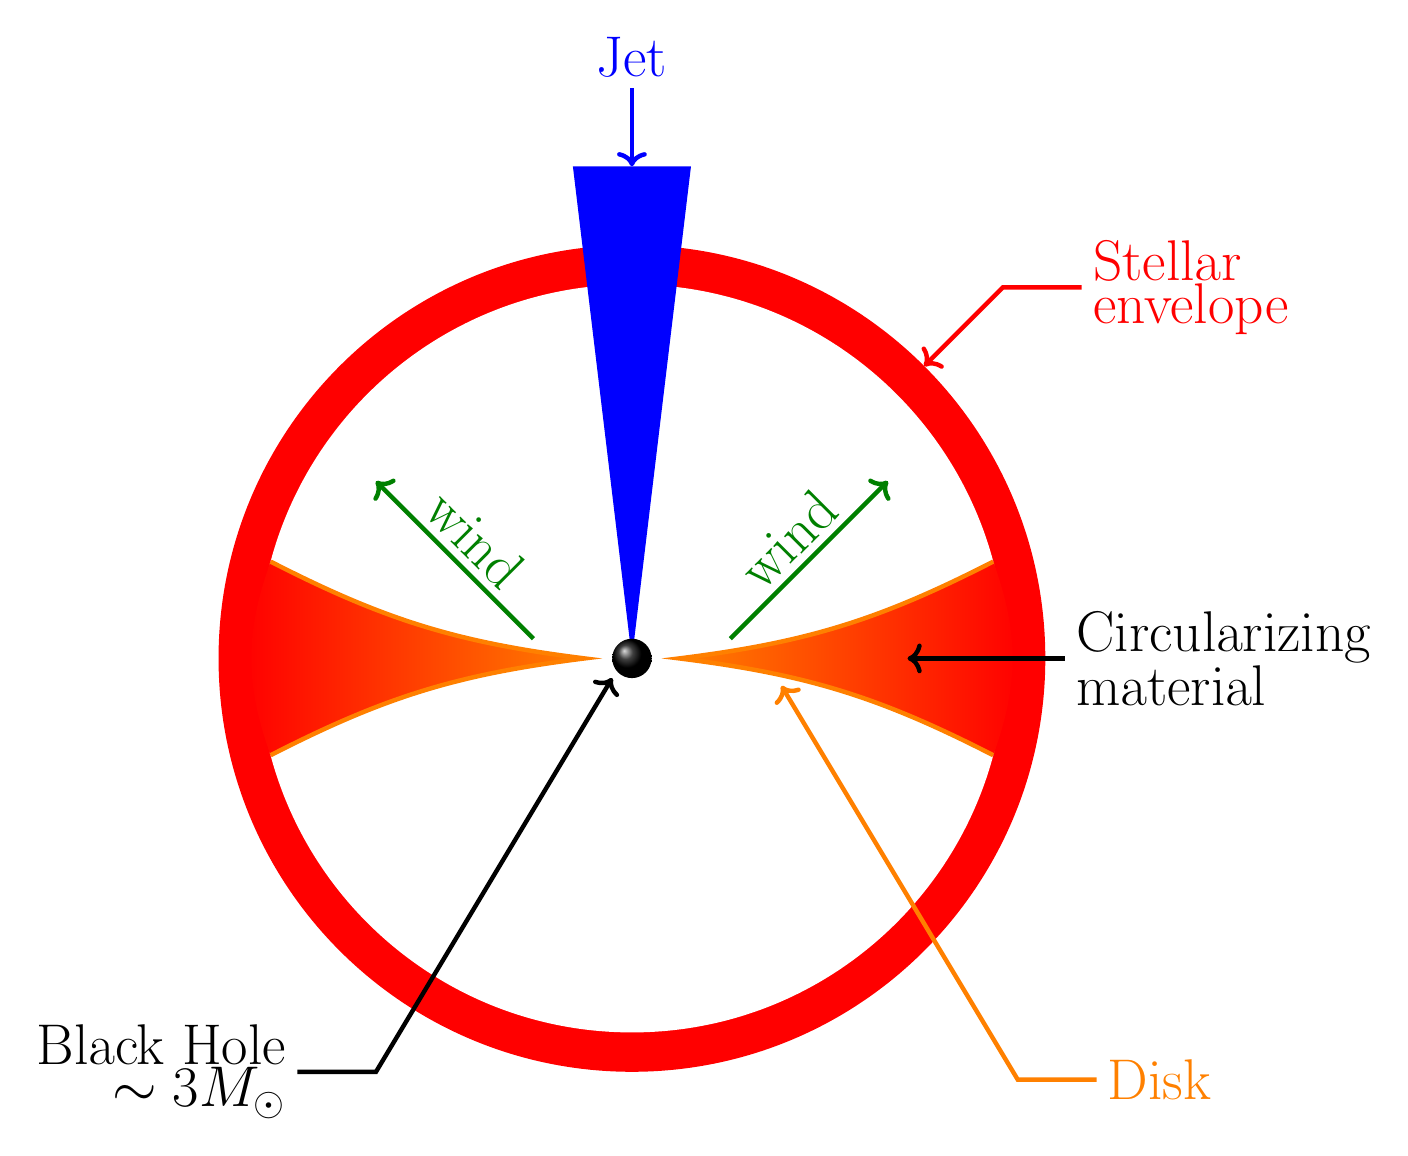
\begin{tikzpicture}
          \coordinate (origin) at (0,0);
          \pgfmathsetmacro{\pi}{3.14159}
          \pgfmathsetmacro{\dbx}{0.5}
          \pgfmathsetmacro{\dby}{0.05}
          \pgfmathsetmacro{\dex}{2.}
          \pgfmathsetmacro{\dey}{0.25}
          \pgfmathsetmacro{\dcc}{2.1}
          \pgfmathsetmacro{\tcx}{5.0}
          \pgfmathsetmacro{\rstar}{5}
          \pgfmathsetmacro{\wstar}{0.25}
          \pgfmathsetmacro{\wjet}{0.75}
          \pgfmathsetmacro{\tangle}{{45}}
          \pgfmathsetmacro{\tsx}{{(\rstar+\wstar)*cos(\tangle)}}
          \pgfmathsetmacro{\tsy}{{(\rstar+\wstar)*sin(\tangle)}}

          \pgfmathsetmacro{\cangle}{15}
          \pgfmathsetmacro{\cx}{(\rstar-\wstar)*cos(\cangle)}
          \pgfmathsetmacro{\cy}{(\rstar-\wstar)*sin(\cangle)}
          % \pgfmathsetmacro{\cend}{\dex + 0.1}
          \pgfmathsetmacro{\cend}{\dbx + 0.1}

          \newcommand{\msize}{\huge}

          % star
          \fill [color=red] (origin) circle (\rstar+\wstar);
          \fill [color=white] (origin) circle (\rstar-\wstar);

          % circularization
          \fill[color=red,
          left color=orange,
          middle color=orange,
          right color=red]
          (\cx,\cy) to [bend left=10] (\cend,0)
          to [bend left=10] (\cx,-\cy)
          to [bend right=20] cycle;
          
          \draw[orange,ultra thick]
          (\cx,\cy) to [bend left=10] (\cend, 0)
          to [bend left=10] (\cx,-\cy);

          \fill[color=red,
          right color=orange,
          middle color=orange,
          left color=red]
          (-\cx,\cy) to [bend right=10] (-\cend,0)
          to [bend right=10] (-\cx,-\cy)
          to [bend left=20] cycle;
          
          \draw[orange,ultra thick]
          (-\cx,\cy) to [bend right=10] (-\cend, 0)
          to [bend right=10] (-\cx,-\cy);

          % \foreach \i in {-1,1}
          % {
          %   % disk
          %   \fill[color=orange]
          %   (\i*\dbx,\dby) -- (\i*\dex,\dey)
          %   .. controls (\i*\dcc,0) .. (\i*\dex,-\dey)
          %   -- (\i*\dbx,-\dby) -- cycle;
          % }
          
          % jet
          \fill[color=blue] (origin) -- (-\wjet,1.25*\rstar) -- ++(2*\wjet,0) -- cycle;

          % bh
          \shade[ball color=black] (origin) circle (0.25);

          % wind
          \draw[deepgreen,ultra thick, ->]
          ({0.5*(\dbx + \dex)},\dey) -- ++(2,2);
          \draw ({0.5*(\dbx + \dex) + 1},{(\dey+1)})
          node[above,align=center,rotate=45]
          {\color{deepgreen}\msize wind};
          \draw[deepgreen,ultra thick, ->]
          ({-0.5*(\dbx + \dex)},\dey) -- ++(-2,2);
          \draw ({-(0.5*(\dbx + \dex) + 1)},{(\dey+1)})
          node[above,align=center,rotate=-45]
          {\color{deepgreen}\msize wind};          

          % text
          \draw[<-,orange, ultra thick] (\dex-0.1,-\dey-0.1)
          -- ++(3,-5) -- ++(1,0)
          node[right,align=left]
          {\msize \color{orange}Disk};
          
          \draw[<-,black, ultra thick] (-0.25,-0.25)
          -- ++(-3,-5) -- ++(-1,0)
          node[left,align=right]
          {\msize \color{black}Black Hole\\ \msize $\sim 3 M_{\odot}$};
          
          \draw[<-,red,ultra thick] (\tsx,\tsy)
          -- ++(1,1) -- ++(1,0)
          node[right,align=left]
          {\msize \color{red} Stellar\\ \msize envelope};

          \draw[<-,blue,ultra thick] (0, 1.25*\rstar) -- ++(0,1)
          node[above,align=center] {\msize \color{blue} Jet};

          \draw[<-,black,ultra thick]
          ({0.5*(\dex+\rstar)},0) -- ++(2,0) node[right,align=left]
          {\msize Circularizing\\ \msize material};
          
          \let\msize\undefined
        \end{tikzpicture}
      }
    \end{column}
    \end{columns}
\end{frame}

\begin{frame}
  \frametitle{Neutrino Transport Matters!}
  \begin{center}
    \includegraphics[height=0.8\textheight]{leptoneq/frame_0001}
  \end{center}
  \begin{tiny}
    \textbf{JMM}, B. R. Ryan, J. C. Dolence. ApJS \textbf{241} 30 (2019) 
  \end{tiny}
\end{frame}

\begin{frame}
  \frametitle{Neutrino Transport Matters!}
  \begin{center}
    % \includegraphics[height=0.8\textheight]{leptoneq/frame_0001}
    \animategraphics[height=0.8\textheight,every=5,autoplay,loop,controls]
    {5}{leptoneq/frame_}{0001}{0101}
  \end{center}
  \begin{tiny}
    \textbf{JMM}, B. R. Ryan, J. C. Dolence. ApJS \textbf{241} 30 (2019) 
  \end{tiny}
\end{frame}

\begin{frame}
  \frametitle{The Relevant Conservation Laws}
  \begin{itemize}
  \item Neutrino Transport Equation (assumes massless)
    \begin{small}
      \begin{displaymath}
        {\color{red}\frac{D}{d\lambda}}\paren{\frac{h^3\Inuf}{\eepsilon^3}}
        = \paren{\frac{h^2{\color{blue}\etanuf}}{\eepsilon^2}}
        - \paren{\frac{\eepsilon {\color{blue}\chinuf}}{h}} \paren{\frac{h^3\Inuf}{\eepsilon^3}}
      \end{displaymath}
    \end{small}
  \item Momentum and Internal Energy Conservation
    \begin{small}
      \begin{displaymath}
        \partial_t\sqrbrace{{\color{red}\detg} \paren{T^t_{\ \nu} + \rho_0u^t \delta^t_\nu}}
        + \partial_i\sqrbrace{{\color{red}\detg}\paren{T^i_{\ \nu} + \rho_0 u^i \delta^t_\nu}}
        = {\color{red}\detg} \paren{T^\kappa_{\ \lambda} {\color{red}\Gamma^\lambda_{\nu\kappa}} + {\color{blue}G_\nu}}
      \end{displaymath}
    \end{small}
  \item Electron Number
    \begin{small}
      \begin{displaymath}
        \partial_t\paren{{\color{red}\detg}\rho_0 Y_e u^t}
        + \partial_i\paren{{\color{red}\detg}\rho_0Y_eu^i}
        = {\color{red}\detg} {\color{blue}G_{\text{ye}}}
      \end{displaymath}
    \end{small}
  \item Spacetime (actually much more complicated)
    \begin{small}
      \begin{eqnarray}
        {\color{red}(\partial_t - \mathcal{L}_\beta) \gamma_{ij}} &=& -2{\color{red}\alpha K_{ij}}\nonumber\\
        {\color{red}(\partial_t - \mathcal{L}_\beta) K_{ij}} &=& {\color{red}R_{ij}} + \cdots + 4\pi \left[{\color{blue}(S-\rho)}{\color{red}\gamma_{ij}} - 2{\color{blue} S_{ij}}\right]\nonumber
      \end{eqnarray}
    \end{small}
  \item And baryon number and magnetic flux conservation...
  \end{itemize}
\end{frame}

\begin{frame}
  \frametitle{Why is Transport Hard?}
  \begin{columns}
    \begin{column}{8cm}
      \begin{itemize}
      \item Fluid Equations:
        \begin{itemize}
        \item Variables, e.g., $\rho$, depend on 3 spatial dimensions
          and time:\\
          $\sim \frac{1}{\Delta t} \frac{1}{\Delta x}\frac{1}{\Delta y}\frac{1}{\Delta z} \sim {\color{blue}\left(\frac{1}{\Delta x}\right)^4}$
        \end{itemize}
      \item Boltzmann/Transport equation:
        \begin{itemize}
        \item Variables, e.g., $f$, depend on 3 spatial dimensions, 3 momentum dimensions, and time.
        \item Where am I and where am I going?\\
          $\sim \left(\frac{1}{\Delta t}\right)\left(\frac{1}{\Delta x}\right)^3\left(\frac{1}{\delta p_x}\right)^3$\\
          $\sim {\color{red}\left(\frac{1}{\Delta x}\right)^7}$
        \end{itemize}
      \end{itemize}
    \end{column}
    \begin{column}{4cm}
      \begin{center}
        \resizebox{!}{7.5cm}{
          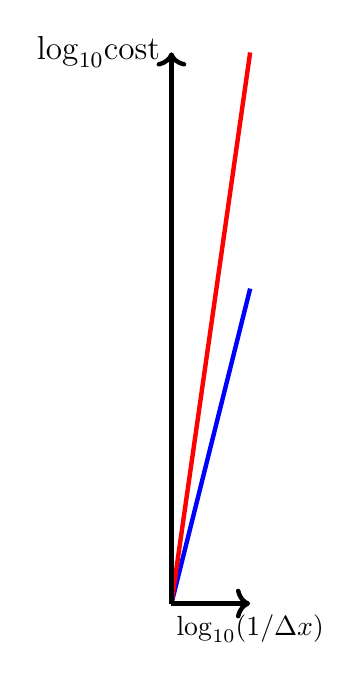
\begin{tikzpicture}[domain=0:1]
            \draw[ultra thick, blue] plot (\x, {4*\x});
            \draw[ultra thick, red] plot (\x, {7*\x});
            \draw[ultra thick,black,->] (0,0) -- (1, 0) node[below] {$\log_{10}(1/\Delta x)$};
            \draw[ultra thick,black,->] (0,0) -- (0, 7) node[left] {\large $\log_{10}$cost};
          \end{tikzpicture}
        }
      \end{center}
    \end{column}
  \end{columns}
\end{frame}

\begin{frame}
  \frametitle{Relevant Neutrino Interactions}
  \begin{tiny}
    \begin{tabular}{l | l | l }
    \hline
    \textbf{Type}&\textbf{Processes}&\textbf{Corrections/Approximations}\\
    \hline
    % \textbf{Emission}&&\\
    \hline
    Abs./Emis. on Neutrons & 
                             \begin{tabular}{@{}l@{}}
                               $\nu_e + n \leftrightarrow e^- + p$\\
                               $\nu_\mu + n \leftrightarrow \mu^- + p$
                             \end{tabular}
                 & 
                             \begin{tabular}{@{}l@{}}
                               Blocking/Stimulated
                               Abs.\\
                               Weak
                               Magnetism\\
                               Recoil
                             \end{tabular}\\
    \hline
    Abs./Emis. on Protons & 
                            \begin{tabular}{@{}l@{}}
                              $\bar{\nu}_e + p \leftrightarrow e^+ +
                              n$\\
                              $\bar{\nu}_\mu + p \leftrightarrow \mu^+
                              + n$\\
                            \end{tabular}
                 & 
                             \begin{tabular}{@{}l@{}}
                               Blocking/Stimulated
                               Abs.\\
                               Weak
                               Magnetism\\
                               Recoil
                             \end{tabular}\\
    \hline
    Abs./Emis. on Ions & $\nu_eA \leftrightarrow A'e^-$ & 
                                                                    \begin{tabular}{@{}l@{}}
                                                                      Blocking/Stimulated Abs.\\
                                                                      Recoil
                                                                    \end{tabular}\\
    \hline
    Electron Capture on Ions & $e^- + A \leftrightarrow A' + \nu_e$ &
                                                                                \begin{tabular}{@{}l@{}}
                                                                                  Blocking/Stimulated Abs.\\
                                                                                  Recoil
                                                                                \end{tabular}\\
                                                             
    \hline
    $e^+-e^-$ Annihilation & $e^+e^- \leftrightarrow \nu_i\bar{\nu}_i$&
                                                                    \begin{tabular}{@{}l@{}}
                                                                      single-$\nu$
                                                                      Blocking\\
                                                                      Recoil
                                                                    \end{tabular}\\
    \hline
    $n_i$-$n_i$ Brehmsstrahlung & $n_i^1 + n_i^2 \to n_i^3 +
                                      n_i^4 + \nu_i\bar{\nu}_i$ 
                                    & 
                                                \begin{tabular}{@{}l@{}}
                                                  single-$\nu$ Blocking\\
                                                  Recoil
                                                \end{tabular}\\
      \hline
      Proton scattering & $\nu_i + p \leftrightarrow \nu_i + p$
                                    & elastic/inelastic\\
      \hline
      Neutron scattering & $\nu_i + n \leftrightarrow \nu_i + n$
                                    & elastic/inealstic\\
      \hline
      Heavy ion scattering & $\nu_i + A \leftrightarrow \nu_i + A$
                                    &
                                      \begin{tabular}{@{}l@{}}
                                        ion-ion correlation\\
                                        electron polarization\\
                                        form-factor
                                      \end{tabular}\\
      \hline
    \end{tabular}
  \end{tiny}
  \begin{itemize}
  \item And this is ignoring Neutrino oscillations!
  \end{itemize}
  {\footnotesize Burrows, Reddy, Thompson, NPA \textbf{177}, 356, (2006)}
\end{frame}

\begin{frame}
  \frametitle{Transport Limits}
  \begin{itemize}
  \item Characterized by optical depth $\tau$ s.t. $I_\nu = I_{\nu}(s_0) e^{-\tau (s_0, s)}$
    \begin{itemize}
    \item Effective ``scattering optical depth'' also matters
    \end{itemize}
  \end{itemize}
  \vspace{1cm}
  \resizebox{12cm}{!}{
    \begin{tikzpicture}
    \draw[ultra thick, black, ->] (0,0) -- ++(8,0);
      % node[below] {$\tau$};

      \node[above,inner sep=0pt] at (0,0.25)
      {\includegraphics[height=1.5cm]{The_Sun_by_the_Atmospheric_Imaging_Assembly_of_NASA's_Solar_Dynamics_Observatory.jpg}};

      \node[above,inner sep=0pt] at (8,0.25)
      {\includegraphics[height=1.5cm]{ns-manhattan}};

      \node[above,inner sep=0pt] at (4,0.25)
      {\includegraphics[height=1.5cm]{disk_image_no_text}};

      \node[below,align=center] at (0,-0.25)
      {$\tau \ll 1$\\free-streaming};

      \node[below,align=center] at (8,-0.25)
      {$\tau \gg 1$\\diffusion};

      \node[below,align=center] at (4,-0.25)
      {Must solve\\full Boltzmann\\Equation};

    \end{tikzpicture}
  }
\end{frame}

\begin{frame}
  \frametitle{How Much Does Transport Matter for disks?}
  \begin{itemize}
  \item Interactions scaling/nucleon:
    \begin{itemize}
    \item $T^6$ typical in disks. Can be as sharp as $T^8$!
    \end{itemize}
  \end{itemize}
  \resizebox{12cm}{!}{
    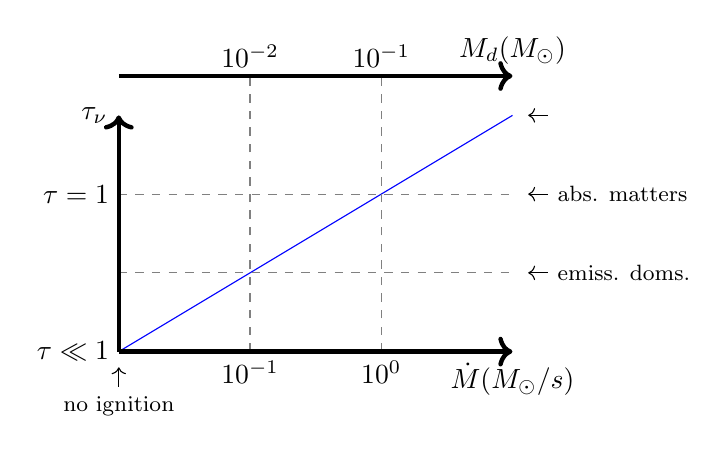
\begin{tikzpicture}
      \coordinate (origin) at (0,0);
      
      \draw[blue] (origin) -- (5,3);

      \node[left] (tau1) at (0,2) {$\tau=1$};
      \draw[dashed,gray] (tau1) -- ++(5.5,0);

      \node[below] (m1) at (10./3.,0) {$10^0$};
      \draw[dashed,gray] (m1) -- ++(0,3.75)
      node[above] {\color{black}$10^{-1}$};

      \coordinate(tau2) at (0,1);
      \draw[dashed,gray] (tau2) -- ++(5,0);

      \node[below](m2) at (5./3.,0) {$10^{-1}$};
      \draw[dashed, gray] (m2) -- ++(0, 3.75)
      node[above] {\color{black}$10^{-2}$};

      \node[left] at (origin) {$\tau\ll 1$};
      \draw[ultra thick, black,->] (origin)
      -- ++(5, 0) node[below] {$\dot{M} (M_\odot/s)$};
      \draw[ultra thick, black, ->] (origin)
      -- ++(0, 3) node[left] {$\tau_\nu$};
      \draw[ultra thick, black, ->] (0,3.5)
      -- ++(5,0) node[above] {$M_d (M_\odot)$};

      \draw[<-] (5.2,3) -- ++(0.25,0);
      \draw[<-] (5.2,2) -- ++(0.25,0) node[right,align=left]
      {\footnotesize abs. matters};

      \draw[<-] (5.2,1) -- ++(0.25,0) node[right,align=left]
      {\footnotesize emiss. doms.};

      \draw[<-] (0,-0.2) -- ++(0,-0.25) node[below,align=center]
      {\footnotesize no ignition};
    \end{tikzpicture}
  }
\end{frame}

\begin{frame}
  \frametitle{Transport Techniques}
  A zoo of techniques with various trade-offs
  \begin{columns}
    \begin{column}{6cm}
      \begin{itemize}
      \item Mesh-based methods, also called Short Characteristics
        \begin{itemize}
        \item {\color{red}More expensive without some notion of sparsity or adaptivity}
        \item Discrete ordinates, also called $S_N$
        \item Finite Elements
        \item Finite Volumes
        \item Finite Differences
        \item Sparse grids
        \end{itemize}
      \end{itemize}
    \end{column}
    \begin{column}{6cm}
      \begin{itemize}
        \item Mesh-free, also called Long Characteristics
          \begin{itemize}
          \item {\color{red}Often shot noise limited}
          \item Ray tracing
          \item Monte Carlo
          \end{itemize}
      \item Approximate methods
        \begin{itemize}
        \item {\color{red}Approximation may or may not be appropriate}
        \item Cooling functions
        \item Leakage
        \item Flux-limited Diffusion
        \item Analytic moment closures
        \end{itemize}
      \item Hybrid methods
        \begin{itemize}
        \item {\color{red}Potentially the best way to navigate the trade-space}
        \end{itemize}
      \end{itemize}
    \end{column}
  \end{columns}
\end{frame}

\begin{frame}
  \frametitle{Technique: Leakage and Cooling}
  \begin{columns}
    \begin{column}{6cm}
      \begin{itemize}
      \item Apply source terms but don't model radiation field
      \item Leakage corrects source terms by trying to account for re-absorption
      \item Requires calculation of optical depth
      \item Relatively simple to implement, potentially faster
      \end{itemize}
    \end{column}
    \begin{column}{6cm}
      \begin{center}        
        \includegraphics[height=7cm]{harm3dnuc_tau}\\
        {\footnotesize Murguia-Berthier et al., ApJ \textbf{919}, 2 (2021)}
      \end{center}
    \end{column}
  \end{columns}
\end{frame}

\begin{frame}
  \frametitle{Technique: Diffusion + Moments}
  \begin{itemize}
  \item Evolve \textit{conserved} quantities of radiation field
    \begin{itemize}
    \item Zeroth moment only: Conserve energy. Radiation field obeys diffusion equation
    \item Zeroth + First moments; Conserve momentum too. Radiation field obeys ``fluid'' equations
    \end{itemize}
  \item Information \textit{lost} by dropping higher-order terms. System must be ``closed.''
  \end{itemize}
  \begin{center}
    \includegraphics[height=4cm]{foucart_moment_v_mc}\\
    {\footnotesize Foucart, MNRAS \textbf{475} 3 (2018)}
  \end{center}
\end{frame}

\begin{frame}
  \frametitle{More compute unlocks short characteristics}
  \begin{columns}
    \begin{column}{6cm}
      \begin{itemize}
      \item Discretize full botlzmann on a grid. Typically in
        spherical coordinates (in momentum space).
      \item ``Classic'' discretization is finite differences $S_N$
      \item Finite volumes discretization (right)
      \item Finite elements discretization (see e.g., work by Maitraya
        Bhattacharya and David Radice)
      \item Sparsity such as sparse grids/tensor networks promising path forward
      \end{itemize}
    \end{column}
    \begin{column}{6cm}
      \begin{center}
        \includegraphics[width=\columnwidth]{mullen_bh_beam}\\
        {\footnotesize White et al., arXiv:2302.04283}
      \end{center}
    \end{column}
  \end{columns}
\end{frame}

\begin{frame}
  \frametitle{A brief aside on Hybrid Methods}
  \begin{itemize}
  \item Moment method closed with full transport solution or analytic
    solution, depending on region of interest
  \item Combines advantages of both approximate and exact methods, at
    cost of particles
  \item See, e.g., Foucart, MNRAS \textbf{475} 3 (2018); Izquierdo et al., 2024
  \end{itemize}
  \begin{center}
    \includegraphics[width=\textwidth]{mocmc-diagram};
  \end{center}
  {\footnotesize Ryan and Dolence, ApJ \textbf{891} 118, (2020).}
\end{frame}

\begin{frame}
  \frametitle{Technique: Particles + Monte Carlo}
  \begin{itemize}
  \item Assume distribution function described by sum over delta functions:
    $$f = \sum_{i=1}^N w_i \delta^3(x - x_i) \delta^3(p - p_i) \delta(t - t_i)$$
  \item Weight $w_i$ for a given particle is the number of
    \textit{physical} particles a single Monte Carlo packet (sometimes
    called \textit{superphoton}) represents.
  \item For technical reasons, can struggle with large optical depths.
    \begin{columns}
      \begin{column}{6.5cm}
        \vspace{-2cm}
        \begin{itemize}
        \item A \textit{fundamentally statistical} approach. Meaningful
          predictions recovered by \textit{integration} over $f$.
        \item Error scales as $1/\sqrt{N}$, no matter number of dimensions!
        \end{itemize}
      \end{column}
      \begin{column}{5.5cm}
        \begin{center}
          \includegraphics[width=\columnwidth]{payel/60-70km_fast_flavor_equator_radial}\\
          {\tiny Mukhopadhyay, \textbf{JMM}, McLaughlin, ArXiv:2404.17938}
        \end{center}
      \end{column}
    \end{columns}
\end{itemize}
\end{frame}

\begin{frame}
  \frametitle{Monte Carlo Transport Basics}
  Interactions with the gas are \textit{probabilistic.}
  \begin{itemize}
  \item Weights $w_i$ chosen at particle emission to fix number of particles
    created in a time step, and thus accuracy/cost:
    $$N_{s,t} = \Delta t \sum_f \int \sqrt{-g}d^3 x d\nu d\Omega \frac{1}{w} \frac{j_{\epsilon,f}}{h\nu}$$
  \item Created particle direction, energy, sampled from emissivity, treating it as a pdf.
  \end{itemize}
  \begin{block}{Gotcha!}
    Resolution controls are heuristic and maintaining appropriate
    resolution can be a problem dependent puzzle. Expect growing
    pains.
  \end{block}
\end{frame}

\begin{frame}
  \frametitle{Scattering and Absorption}
  Also probabilistic. But can be \textit{biased}
  \begin{itemize}
  \item Important for accurately sampling scattering processes!
  \item Can be used to \textit{de-enhance} too. Can stabilize in, e.g., a neutron star.
  \end{itemize}
  \begin{columns}
    \begin{column}{5cm}
      \begin{itemize}
      \item For absorption:
        $$\Delta \tau_a > - \ln(r_a)$$
      \item For scattering:
        $$\Delta \tau_p > -\ln(r_s)/b_s(\nu, f, p)$$
      \item For scattering to play a \textit{fair game}, particles
        \textit{split} upon scattering.
      \end{itemize}
    \end{column}
    \begin{column}{7cm}
      \begin{center}
        \includegraphics[width=\columnwidth]{multiscatt}
      \end{center}
      {\tiny \textbf{JMM}, B. R. Ryan, J. C. Dolence. ApJS \textbf{241} 30 (2019)}
    \end{column}
  \end{columns}
\end{frame}

\begin{frame}
  \frametitle{Gotcha! Tetrads ands Units}
  \begin{columns}
    \begin{column}{6cm}
      \begin{itemize}
      \item Tetrads
      \begin{itemize}
      \item Above interactions all expressed in \textit{Minkowski} space, where algebra is simpler
      \item To get away with this, we transform into a \textit{tetrad}
        frame comoving with the fluid to process radiation-matter
        interactions
      \end{itemize}
    \item Units
      \begin{itemize}
      \item GR frequently scale-free.
      \item Matter-radiation interactions not scale-free. CGS is natural.
      \item Do ``lab-frame'' physics in natural units. Move to CGS to
        process, e.g., emissivity.
      \end{itemize}
      \end{itemize}
    \end{column}
    \begin{column}{6cm}
      \resizebox{6cm}{!}{
        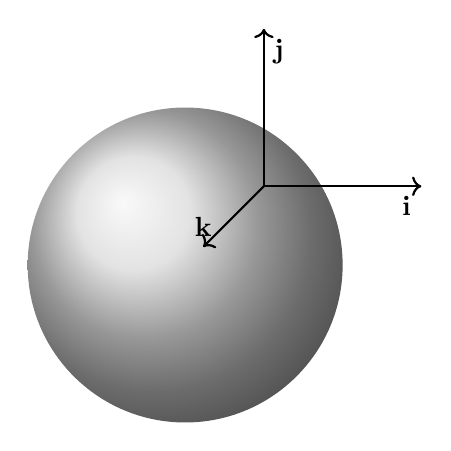
\begin{tikzpicture}
          % Draw the disk
          \shade[ball color=gray!30] (-1,-1) circle (2cm);
          
          % Draw the axes
          \draw[thick,->] (0,0,0) -- (2,0,0) node[anchor=north east] {$\mathbf{i}$};
          \draw[thick,->] (0,0,0) -- (0,2,0) node[anchor=north west] {$\mathbf{j}$};
          \draw[thick,->] (0,0,0) -- (0,0,2) node[anchor=south] {$\mathbf{k}$};
                  \end{tikzpicture}
      }
    \end{column}
  \end{columns}
\end{frame}

\begin{frame}
  \frametitle{Particle Motion}
  \begin{columns}
    \begin{column}{6cm}
      \begin{itemize}
      \item Particle paths evolved \textit{deterministically}:
        $$\frac{d^2 x^\mu}{d\lambda^2} + \Gamma^\mu_{\alpha\beta} \frac{d x^\mu}{d\lambda} \frac{d x^\nu}{d \lambda} = 0$$
      \item Assume neutrinos are massless (not quite true but good enough)
      \end{itemize}
    \end{column}
    \begin{column}{6cm}
      \begin{center}
        \includegraphics[width=\columnwidth]{grmonty_geodesics}\\
        {\tiny Dolence et al., (2009) ApJS \textbf{184} 387}
      \end{center}
    \end{column}
  \end{columns}
\end{frame}

\begin{frame}
  \frametitle{Putting it all together in $\nu\texttt{bhlight}$!}
  \begin{itemize}
  \item \textbf{Magnetized gas} via \textit{finite volume methods}
    \begin{itemize}
    \item Standard second-order Gudonov scheme
    \item Cell-centered constrained transport for magnetic fields
    \item WENO5 reconstruction
    \item Local Lax-Friedrichs Riemann solver
    \end{itemize}
  \item \textbf{Neutrinos} via \textit{Monte Carlo methods}
    \begin{itemize}
    \item Explicit integration along geodesics
    \item Probabilistic emissivity, absorption, and scattering
    \item Novel biasing scheme ensures all processes well-sampled
    \end{itemize}
  \item \textbf{Coupled} via \textit{operator splitting}
  \item Built on top of $\texttt{HARM}$, $\texttt{grmonty}$, and
    $\texttt{bhlight}$.
  \end{itemize}
\end{frame}

\begin{frame}
  \frametitle{The August 2017 Disk}
  \begin{center}
    % \includegraphics[height=0.475\textheight]{gw170817disk_Ye_close/frame_0831} \\
    % \includegraphics[height=0.475\textheight]{gw170817disk_Ye_far/frame_0831} 
    \animategraphics[height=0.475\textheight,every=5,autoplay,loop,controls=off]
    {10}{gw170817disk_Ye_close/frame_}{0001}{0837} \\
    \animategraphics[height=0.475\textheight,every=5,autoplay,loop,controls=off]
    {10}{gw170817disk_Ye_far/frame_}{0001}{0837} 
  \end{center}
  %\textbf{JMM}+, in prep.
\end{frame}

\begin{frame}
  \frametitle{Exquisite Access to the Radiation Field}
  \begin{center}
    % \includegraphics[width=0.9\textwidth]{nphys_frames/frame_00531}
    \animategraphics[width=0.9\textwidth,every=10,autoplay,loop,controls=off]
    {20}{nphys_frames/frame_}{00001}{00965}
  \end{center}
  \begin{tiny}
    \textbf{JMM} et al. PRD \textbf{100} 023008 (2019)
  \end{tiny}
\end{frame}

\begin{frame}
  \frametitle{Electron Fraction of the Outflow}
  \begin{columns}
    \begin{column}{6cm}
      \includegraphics[height=0.9\textheight]{gw170817-ye-vs-theta-folded-5}\\
      \begin{tiny}
        \textbf{JMM} et al. PRD \textbf{100} 023008 (2019)
      \end{tiny}
    \end{column}
    \begin{column}{6cm}
      \resizebox{\columnwidth}{!}{
        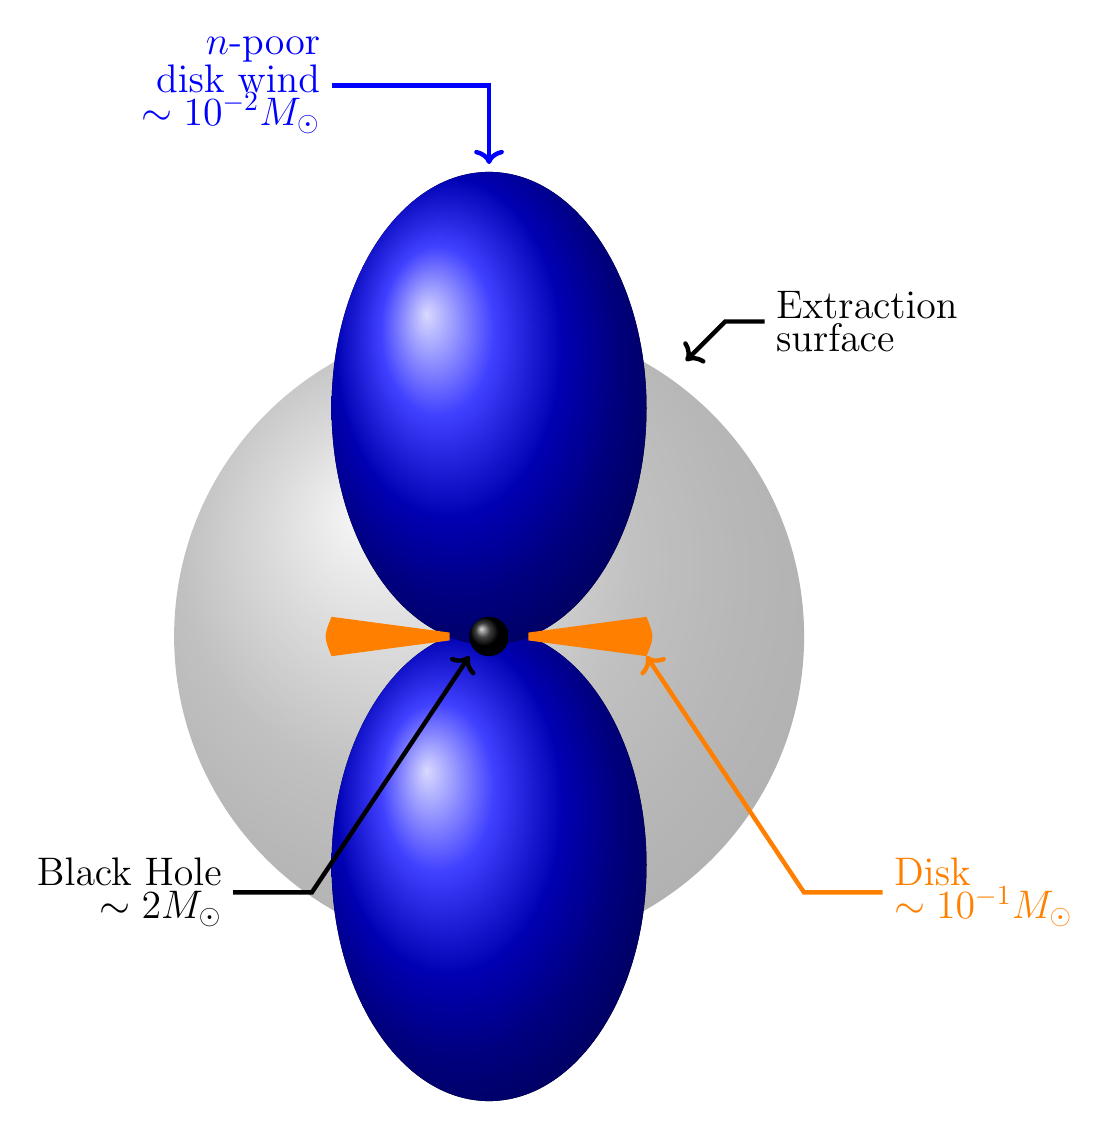
\begin{tikzpicture}
          \tikzfading[name=fade inside,
          inner color=transparent!50,
          outer color=transparent!50]
          
          \coordinate (origin) at (0,0);
          \pgfmathsetmacro{\dbx}{0.5}
          \pgfmathsetmacro{\dby}{0.05}
          \pgfmathsetmacro{\dex}{2.}
          \pgfmathsetmacro{\dey}{0.25}
          \pgfmathsetmacro{\dcc}{2.1}
          \pgfmathsetmacro{\tcx}{5.0}
          
          % extraction surface
          \shade[ball color=gray,path fading=fade inside,opacity=0.75] (origin) circle (4);

          \foreach \i in {-1,1}
          {
            \fill[ball color=blue] (0, \i*2.9) ellipse (2 and 3);
          }
          
          \foreach \i in {-1,1}
          {
            % disk
            \fill[color=orange]
            (\i*\dbx,\dby) -- (\i*\dex,\dey)
            .. controls (\i*\dcc,0) .. (\i*\dex,-\dey)
            -- (\i*\dbx,-\dby) -- cycle;
          }
          
          % bh
          \shade[ball color=black] (origin) circle (0.25);
                    
          % text
          \draw[<-,blue, ultra thick] (0,6) -- ++(0,1) -- ++(-2,0)
          node[left,align=right]
          {\Large \color{blue}$n$-poor\\\Large disk wind\\\Large $\sim 10^{-2}M_{\odot}$};
          
          \draw[<-,orange, ultra thick] (\dex,-\dey)
          -- ++(2,-3) -- ++(1,0)
          node[right,align=left]
          {\Large \color{orange}Disk\\\Large $\sim 10^{-1}M_{\odot}$};
          
          \draw[<-,black, ultra thick] (-0.25,-0.25)
          -- ++(-2,-3) -- ++(-1,0)
          node[left,align=right]
          {\Large \color{black}Black Hole\\ \Large $\sim 2 M_{\odot}$};

          \draw[<-,black,ultra thick] (2.5,3.5)
          -- ++(0.5,0.5) -- ++(0.5,0) node[right,align=left]
          {\Large \color{black}Extraction\\\Large surface};
        \end{tikzpicture}
      }
    \end{column}
  \end{columns}
\end{frame}

\begin{frame}
  \frametitle{Nucleosynthesis}
  \begin{columns}
    \begin{column}{9cm}
      \begin{center}
        \includegraphics[width=\columnwidth]{gw170817-yields-2}
      \end{center}
      \begin{tiny}
        \textbf{JMM} et al. PRD \textbf{100} 023008 (2019)
      \end{tiny}
    \end{column}
    \begin{column}{3cm}
      \begin{itemize}
      \item r-process networks:
        \begin{itemize}
        \item SkyNet
        \item PRISM
        \item CFNET
        \item etc.
        \end{itemize}
      \end{itemize}
    \end{column}
  \end{columns}
\end{frame}

\begin{frame}
  \frametitle{Spectra}
  \begin{center}
    \includegraphics[width=\columnwidth]{spectral_evolution}
  \end{center}
  \begin{tiny}
    \textbf{JMM} et al. PRD \textbf{100} 023008 (2019)
  \end{tiny}
\end{frame}

\begin{frame}
  \frametitle{Cool Science to Do}
  \begin{columns}
    \begin{column}{6cm}
      \begin{center}
        \includegraphics[height=3.5cm]{bhns_curtis/nsbh_disks_rho_ye_0}\\
        \includegraphics[height=3.5cm]{bhns_curtis/nsbh_disks_rho_ye_3}
      \end{center}
    \end{column}
    \begin{column}{6cm}
      \begin{itemize}
      \item Model a suite of exotic post-BHNS merger disks
      \end{itemize}
      \begin{center}
        \includegraphics[width=6cm]{bhns_curtis/total_abun_disks_dec22}
        {\footnotesize Curtis, \textbf{JMM}, et al., ApJS 945 L13 (2023)}
      \end{center}
    \end{column}
  \end{columns}
\end{frame}

\begin{frame}
  \frametitle{Impact of Magnetic Field}
  \begin{itemize}
  \item Magnetically-driven turbulence drives angular momentum transport.
  \item \textit{Dr.} Kelsey Lund (defended yesterday!)
  \end{itemize}
  \begin{columns}
    \begin{column}{2.5cm}
      \begin{center}
        \includegraphics[height=6cm]{kelsey/4ms_comp}
      \end{center}
    \end{column}
    \begin{column}{9.5cm}
      \begin{itemize}
      \item Field must ``spin up'' due to turbulent instability.
      \item Larger fields mean less spin-up time, also more ``memory''
        of initial configuration.
      \item Impacts yields, outflow morphology.
      \end{itemize}
      \begin{center}
        \includegraphics[height=3cm]{kelsey/masses_wpercent}
      \end{center}
      {\footnotesize Lund, \textbf{JMM}, et al., (2024) ApJ \textbf{964} 111}
    \end{column}
  \end{columns}
\end{frame}

\begin{frame}
  \frametitle{Ultra Late-Time Outflow}
  \begin{itemize}
  \item Original models of post-merger disks (and collapsars) only run
    for very short time: $\sim 120$ms.
  \item Outflow not finished by this time. Late-time outflow may look
    very different.
  \item Extended simulation to 1.2s physical time. 7 months required
    on supercomputer.
  \end{itemize}
  \begin{columns}
    \begin{column}{6cm}
      \begin{center}
        \includegraphics[width=0.9\columnwidth]{longsim/outflow_components}
      \end{center}
    \end{column}
    \begin{column}{6cm}
      \begin{center}
        \includegraphics[width=0.9\columnwidth]{longsim/ya_short_v_long}
      \end{center}
    \end{column}
  \end{columns}
  {\footnotesize Sprouse, \textbf{JMM}, et al., (2024) ApJ \textbf{962} 79}
\end{frame}

\begin{frame}
  \frametitle{Fast Flavor Transformations}
  \begin{itemize}
  \item Neutrinos can \textit{oscillate} from one flavor to
    another. This can impact nucleosynthesis.
  \item Due to length/time scales, impossible to treat from first principles
  \end{itemize}
  \begin{columns}
    \begin{column}{6cm}
      \begin{center}
        \includegraphics[width=0.9\columnwidth]{payel/60-70km_fast_flavor_equator_radial}
      \end{center}
    \end{column}
    \begin{column}{6cm}
      \begin{center}
        \includegraphics[width=0.9\columnwidth]{payel/crossing_space}
      \end{center}
    \end{column}
  \end{columns}
  {\footnotesize Mukhopadhyay, \textbf{JMM}, McLaughlin, ArXiv:2404.17938}
\end{frame}

\begin{frame}
  \frametitle{Parthenon: Unlocking GPU Cycles}
  \begin{columns}
    \begin{column}{6cm}
      \begin{center}
        \includegraphics[width=\columnwidth,clip,trim={0 0 150 100}]{top500}
      \end{center}
      {\footnotesize Top500 List}
    \end{column}
    \begin{column}{6cm}
      \begin{center}
        \includegraphics[height=6cm]{parth-hydro-scaling_weak}
      \end{center}
      {\footnotesize Grete, \textbf{JMM}, et al., ArXiv:2202.12309}
    \end{column}
  \end{columns}
\end{frame}

\begin{frame}
  \frametitle{Tools built on top of Parthenon}
  \begin{columns}
    \begin{column}{6cm}
      \begin{itemize}
      \item Phoebus, neutron star
      \end{itemize}
      \begin{center}
        \includegraphics[height=6cm]{tov_fig_paper}
      \end{center}
    \end{column}
    \begin{column}{6cm}
      \begin{itemize}
      \item Athena-PK, turbulence
      \end{itemize}
      \begin{center}
        \includegraphics[width=\columnwidth]{athenapk_sample}
      \end{center}
        \begin{itemize}
        \item Riot, triple point
        \end{itemize}
        \begin{center}
          \includegraphics[height=3cm]{triple}
        \end{center}
    \end{column}
  \end{columns}
  {\footnotesize Grete, \textbf{JMM}, et al., ArXiv:2202.12309}
\end{frame}

\begin{frame}
  \frametitle{Next Generation of Full-Transport Disks in Phoebus}
  \begin{columns}
    \begin{column}{6cm}
      \begin{itemize}
      \item \textit{Dr.} Brandon Barker (just defended his thesis)
      \item Current capabilities:
        \begin{itemize}
        \item Curvilinear coordinates
        \item nuclear EOS
        \item Monte Carlo transport
        \item GPUs
        \end{itemize}
      \item Soon to be ready:
        \begin{itemize}
        \item Adaptive mesh refinement
        \end{itemize}
      \end{itemize}
    \end{column}
    \begin{column}{6cm}
      \begin{center}
        % \includegraphics[width=0.9\textwidth]{barker_2d/frame_100}
        \animategraphics[width=0.9\textwidth,every=10,autoplay,loop,controls=off]
        {10}{barker_2d/frame_}{001}{200}
      \end{center}
    \end{column}
  \end{columns}
\end{frame}

\begin{frame}
  \frametitle{Supernovae in Phoebus}
  \begin{itemize}
  \item \textit{Dr.} Mariam Gogilashvili (just defended her thesis)
  \item Connecting pen-and-paper model (FEC) to simulations: Gogilashvili and Murphy, MNRAS \textbf{515} 2, (2022)
  \item Gogilashvili, Murphy, \textbf{JMM}, (2024) ApJ \textbf{962} 110
  \end{itemize}
  \begin{columns}
    \begin{column}{6cm}
      \begin{center}
        % \includegraphics[width=0.9\textwidth]{mgog_1d/frame_500}
        \animategraphics[width=0.9\textwidth,every=20,autoplay,loop,controls=off]
        {20}{mgog_1d/frame_}{001}{900}
      \end{center}
    \end{column}
    \begin{column}{6cm}
      \begin{center}
        \includegraphics[width=\columnwidth]{FECvsTime}
      \end{center}
    \end{column}
  \end{columns}
\end{frame}

\begin{frame}
  \frametitle{Get Involved}
  \begin{itemize}
  \item Parthenon: \url{https://github.com/parthenon-hpc-lab/parthenon}
  \item Phoebus: \url{https://github.com/lanl/phoebus}
  \item $\nu$bhlight: \url{https://github.com/lanl/nubhlight}
  \item singularity-eos: \url{https://github.com/lanl/singularity-eos}
  \item singularity-opac: \url{https://github.com/lanl/singularity-opac}
  \item Spiner: \url{https://github.com/lanl/spiner}
  \end{itemize}
\end{frame}

\begin{frame}
  \frametitle{Summary.}
  \begin{itemize}
  \item Neutron star mergers definitively a source of r-process elements
  \item Mapping merger parameters to observables has many
    uncertainties and degeneracies. Neutrinos are key!
  \item Transport is hard: real transport has been computationally
    intractable until very recently.
  \item We've hit a phase transition. Better computers and better
    numerical methods have converged and model fidelity is improving
    very rapidly.
  \item The future is (neutrino) bright!
  \end{itemize}
\end{frame}

\backupbegin

\begin{frame}
  \frametitle{Accretion Rates}
  \begin{columns}
    \begin{column}{4cm}
      \resizebox{4cm}{!}{
        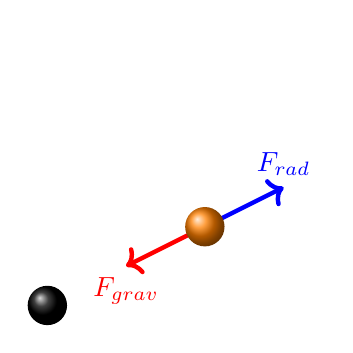
\begin{tikzpicture}
          \tikzfading[name=fade inside,
          inner color=transparent!50,
          outer color=transparent!50]
          
          \coordinate (origin) at (0,0);
          \pgfmathsetmacro{\dbx}{0.5}
          \pgfmathsetmacro{\dby}{0.05}
          \pgfmathsetmacro{\dex}{2.}
          \pgfmathsetmacro{\dey}{0.25}
          \pgfmathsetmacro{\dcc}{2.1}
          \pgfmathsetmacro{\tcx}{5.0}

          % bh
          \shade[ball color=black] (origin) circle (0.25);

          % vectors
          \draw[red, ultra thick,->] (2, 1) -- (1,0.5) node[below] {\color{red} $F_{grav}$};
          \draw[blue, ultra thick, ->] (2, 1) -- (3,1.5) node[above] {\color{blue} $F_{rad}$};

          % particle
          \shade[ball color=orange] (2,1) circle (0.25);

        \end{tikzpicture}
      }
    \end{column}
    \begin{column}{8cm}
      \begin{center}
        \includegraphics[width=0.9\textwidth]{mdot_edd}
      \end{center}
    \end{column}
  \end{columns}
\end{frame}

\begin{frame}
  \frametitle{Accretion Rates}
  \begin{columns}
    \begin{column}{4cm}
      \resizebox{4cm}{!}{
        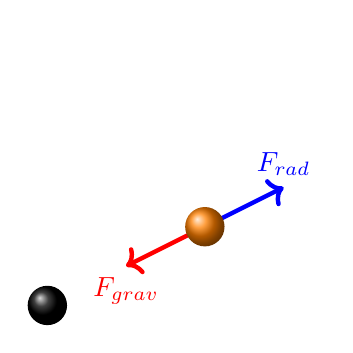
\begin{tikzpicture}
          \tikzfading[name=fade inside,
          inner color=transparent!50,
          outer color=transparent!50]
          
          \coordinate (origin) at (0,0);
          \pgfmathsetmacro{\dbx}{0.5}
          \pgfmathsetmacro{\dby}{0.05}
          \pgfmathsetmacro{\dex}{2.}
          \pgfmathsetmacro{\dey}{0.25}
          \pgfmathsetmacro{\dcc}{2.1}
          \pgfmathsetmacro{\tcx}{5.0}

          % bh
          \shade[ball color=black] (origin) circle (0.25);

          % vectors
          \draw[red, ultra thick,->] (2, 1) -- (1,0.5) node[below] {\color{red} $F_{grav}$};
          \draw[blue, ultra thick, ->] (2, 1) -- (3,1.5) node[above] {\color{blue} $F_{rad}$};

          % particle
          \shade[ball color=orange] (2,1) circle (0.25);

        \end{tikzpicture}
      }
    \end{column}
    \begin{column}{8cm}
      \begin{center}
        \includegraphics[width=0.9\textwidth]{mdot_edd_nu}
      \end{center}
    \end{column}
  \end{columns}
\end{frame}

\begin{comment}
\begin{frame}

\begin{frame}
  \frametitle{Stationary Disk, No Ye equilibrium!}
  \setlength{\unitlength}{1cm}
  \begin{picture}(12,8)
    \visible<1>{
      \put(2, 0.5){
        \includegraphics[height=0.9\textheight]{collapsar/ye_statistics}
      }
    }
    \visible<2->{
      \put(0,1) {
        \includegraphics[width=0.5\textwidth]{collapsar/ye_statistics}
      }
      \put(6,4) {
        \includegraphics[width=0.5\textwidth]{collapsar/rho_Ye_snap_t5000}
      }
      \put(5,0.0) {
        \includegraphics[width=0.6\textwidth]{collapsar/selected_traces_lattitude_cut}
      }
      \put(0,0){
        {\footnotesize Miller et al., ApJ \textbf{902}, 66 (2020)}
      }
    }
  \end{picture}
\end{frame}

\begin{frame}
  \frametitle{Turbulence and $Y_e$}
  \resizebox{12cm}{!}{
    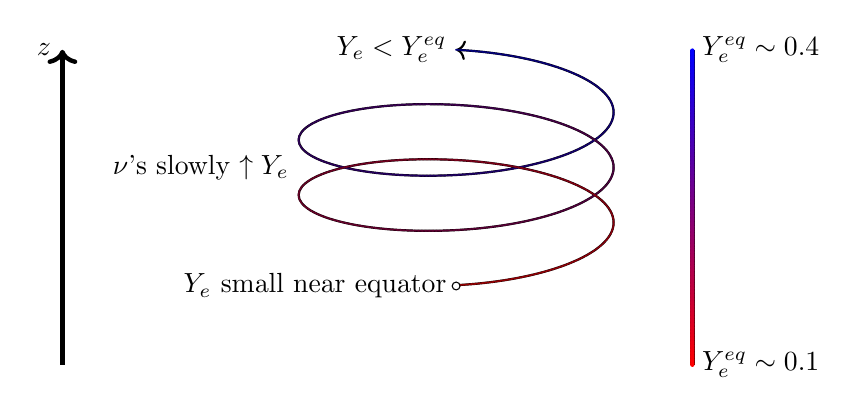
\begin{tikzpicture}
      \coordinate(origin) at (-2,0);

      \draw[ultra thick, black, ->] (origin) -- ++ (0, 4)
      node[left] {$z$};

      \draw[ultra thick,colormorph={0.8pt}{red}{blue}] (6,0) -- ++(0,4);
      \node[right] at (6,0) {$Y_e^{eq}\sim 0.1$};
      \node[right] at (6,4) {$Y_e^{eq}\sim 0.4$};

      \draw[thick,
      decoration={aspect=0.31,segment length=7mm,amplitude=2cm, coil},
      colormorph={0.4pt}{deepblue}{deepred},
      decorate,arrows={<[bend]-}] (3,4) -- (3,1);
      \node[draw,fill=white,circle,inner sep=1pt] at (3,1) {};
      \node[left] at (3,1) {$Y_e$ small near equator};
      \node[left] at (1.,2.5) {$\nu$'s slowly $\uparrow Y_e$};
      \node[left] at (3,4) {$Y_e < Y_e^{eq}$};
    \end{tikzpicture}
  }
\end{frame}

\begin{frame}
  \frametitle{$Y_e$ is set by the balance of Turbulence and
    Neutrinos!}
  \begin{displaymath}
      Y_{\rm e}(z/H) = \braket{\text{min}(Y_{\rm e})}_{\text{trc}}
      + \braket{\frac{d Y_{\rm e}}{dt}}_{t,\text{trc}} \paren{H\braket{\frac{dz}{dt}}_{t,\text{trc}}^{-1}}\paren{\frac{z}{H} - \braket{\text{min}(z/H)}_{\text{trc}}}
    \end{displaymath}
    \begin{columns}
      \begin{column}{6cm}
        \includegraphics[width=\columnwidth]{collapsar/vertical-structure-params}
      \end{column}
      \begin{column}{6cm}
        \includegraphics[width=\columnwidth]{collapsar/model-vs-vertical-structure}
      \end{column}
    \end{columns}
    {\footnotesize Miller et al., ApJ \textbf{902}, 66 (2020)}
\end{frame}
\end{comment}

% \begin{frame}
%   \frametitle{Neutrino Transport}
%   \begin{center}
%     % \includegraphics[height=0.9\textheight]{tau_frames/frame_00531}
%     \animategraphics[height=0.9\textheight,every=10,autoplay,loop,controls=off]
%     {20}{tau_frames/frame_}{00001}{00983}
%   \end{center}
% \end{frame}

\backupend

\end{document}